\documentclass[spanish, 10pt,a4paper]{article}
\usepackage[spanish]{babel}
\usepackage[utf8]{inputenc}
\usepackage{textcomp}
\usepackage{hyperref}
\usepackage[pdftex]{graphicx}
\usepackage{epsfig}
\usepackage{amsmath}
\usepackage{hyperref}
\usepackage{amssymb}
\usepackage{color}
\usepackage{graphics}
\usepackage{amsthm}
\usepackage{caratula}
\usepackage{fancyhdr,lastpage}
\usepackage[paper=a4paper, left=1.4cm, right=1.4cm, bottom=1.4cm, top=1.4cm]{geometry}
\usepackage[table]{xcolor} % color en las matrices
\usepackage[font=small,labelfont=bf]{caption} % caption de las figuras en letra mas chica que el texto
\usepackage[ruled,vlined,linesnumbered]{algorithm2e}
\usepackage{listings}
\usepackage{float}
\usepackage{amsfonts}
\usepackage{upgreek}

\color{black}

%%%PAGE LAYOUT%%%
\topmargin = -1.2cm
\voffset = 0cm
\hoffset = 0em
\textwidth = 48em
\textheight = 164 ex
\oddsidemargin = 0.5 em
\parindent = 2 em
\parskip = 3 pt
\footskip = 7ex
\headheight = 20pt
\pagestyle{fancy}
\lhead{Teor\'ia de la Comunicaciones - 2015 C2 - Trabajo Pr\'actico 2} % cambia la parte izquierda del encabezado
\renewcommand{\sectionmark}[1]{\markboth{#1}{}} % cambia la parte derecha del encabezado
\rfoot{\thepage}
\cfoot{}

%spaced sections



%El siguiente paquete permite escribir la caratula facilmente
\hypersetup{
  pdftitle={ 1c2015.PLP.RTP3},
  colorlinks,
  citecolor=black,
  filecolor=black,
  linkcolor=black,
  urlcolor=black 
}

\materia{Teor\'ia de las Comunicaciones}

\titulo{Trabajo Pr\'actico 2}

\subtitulo{Teor\'ia de las Comunicaciones}

\grupo{Grupo 4}

\integrante{Ignacio Niesz}{722/10}{ignacio.niesz@gmail.com}
\integrante{Leandro Vega}{698/11}{leandrogvega@gmail.com}
\integrante{Rodrigo Cisneros}{920/10}{rodricis@hotmail.com}
\integrante{Santiago Pernigotti}{870/11}{s.a.pernigotti89@gmail.com}
 
\begin{document}
{ \oddsidemargin = 2em
	\headheight = -20pt
	\maketitle	
}
  
	\tableofcontents
	\newpage
	\section{Introducci\'on}

En este trabajo pr\'actico vamos a desarrollar una implementaci\'on propia de traceroute. Traceroute es una consola de diagn\'ostico que permite seguir el recorrido de los paquetes, conocer cada nodo (router) por el que pasa, hasta llegar un host destino. Para poder conocer la ruta que recorren los paquetes e implementarlo, vamos a necesitar tener en cuenta las siguientes herramientas:

\begin{itemize}

\item Scapy: Herramiento usada en el trabajo pr\'actico anterior. Es una utilidad escrita en Python que nos servir\'a para crear y manipular paquetes, escanear, funciones de sniffer, entre otras.

\item ICMP (Internet Control Message Protocol): Es el sub protocolo de control y notificaci\'on de errores del Protocolo de Internet (IP). Se usa para enviar mensajes de error o de control, indicando por ejemplo que un servicio determinado no está disponible, o que un router o host no puede ser localizado, o que un paquete ha llegado al destino.
\begin{figure}[h]
	\begin{center}
    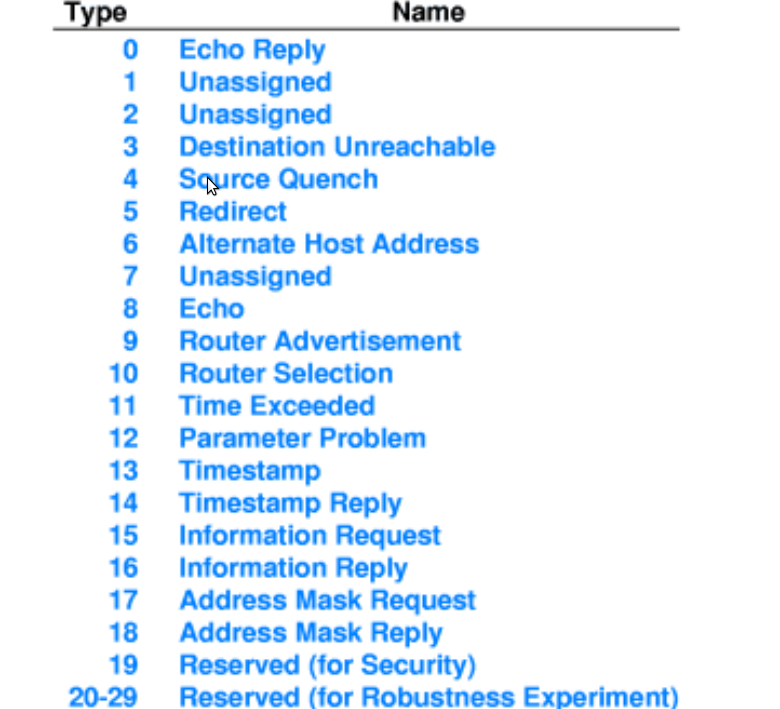
\includegraphics[width=0.5\textwidth]{ICMP_lista.png}
     \label{fig:ICMPlista} 
	\end{center}    
    \caption{Lista de algunos mensajes de control permitidos.}  
    
\end{figure}
\vspace{0.25cm}

\item TTL (time to live): No es mas que el tiempo de vida del paquete. Dentro del paquete enviado se setea dicho valor (entero) para saber cuando un paquete debe ser descartado, en caso que no llegue al destino. La forma en que funciona es: cada vez que el paquete pasa por un nodo, \'este \'ultimo le resta una unidad al valor que ten\'ia cuando lo recibi\'o, y lo propaga al siguiente nodo. En caso que el valor llegue a cero, el nodo descarta dicho paquete evitando que se siga propagando hasta su destino.

\item ICMP y TTL: Si a un paquete se le vence su TTL ($TTL = 0$), y \'este no est\'a en el nodo correspondiente a su host destino, nos llega un mensaje ICMP de "Time Exceeded" ($11$). En caso contrario, si un paquete llego a su host destino, sin importar el valor de su TTL, entonces via ICMP nos llegar\'a un mensaje de ''Echo Replay" ($0$).

\item RTT (Round-Trip delay Time): Es el tiempo que tarda un paquete de datos enviado desde un emisor en volver a este mismo, habiendo pasado por el receptor de destino. Es uno de los datos que nos muestra por pantalla las implementaciones hechas actualmente de traceroute. Con este valor podremos saber cuanto tardan los paquetes en llegar a cada nodo que intervienen en el recorrido hacia el host destino.

\end{itemize}

Una vez logrado el correcto funcionamiento del traceroute, con lo cual podremos conocer toda la ruta de un paquete, debemos tomar las estadísticas pertinentes para satisfacer los pedidos en las consignas dadas en el enunciado. Estos son:

\begin{itemize}

\item RTT promedio: Es lo que tarda un enlace en contestarnos al hacerle varias corridas, tomar diferentes tiempos y promediando dicho valor. Esto nos sirve para estimar el tiempo verdadero que tarda en llegar nuestro paquete hacia ese lugar, mitigando posibles errores en instancias particulares que pudieran darnos fuera de lo normal.

\item $\Delta$RTT: Es la diferencia entre el RTT promedio de un nodo con respecto a su antecesor.

\item Desv\'io Estandar para cada salto: Es la raiz cuadrada de la varianza, la cual nos dice que tan dispersos son los datos tomados.

\item Test de hip\'otesis: Normal test\footnote{\url{https://en.wikipedia.org/wiki/Normal_distribution}} y Grubbs test\footnote{\url{https://en.wikipedia.org/wiki/Grubbs\%27_test_for_outliers}}. Adem\'as, para detectar outliers en el Grubbs test, necesitamos saber si el valor obtenido supera un rango que se deduce mediante t-student\footnote{\url{https://en.wikipedia.org/wiki/Student\%27s_t-distribution}}.

\item Outliers: Son los enlaces submarinos o significativos, los enlaces que tienen un salto relevante con respecto a su antecesor.

\end{itemize}

\subsection{Rutas Universitarias} 

Rutas a universidades por fuera de sudam\'erica: Como la idea que nos proponen, dado el test de Grubbs, es encontrar enlaces con saltos significativos (outliers), hemos optado por elegir universidades de distintos continentes en el cual hayan oc\'eanos de distancia con respecto a nuestra IP localizada en Argentina. Estimando que ante m\'as distancias, posiblemente tengamos saltos significativamente m\'as grandes. Las elegidas son:

\begin{itemize}
\item La Universidad Rusa de la Amistad de los Pueblos (URAP)
\item Universidad de Sydney
\item Universidad de Hamburgo (Alemania)
\end{itemize}
	\newpage
	\section{Desarrollo}


El programa requiere 5 parámetros de entrada:

\begin{itemize}

\item  Host destino: Host para localizar la ruta (puede ser IP o una direccion web)

\item Tiempo límite: Tiempo límite para cortar la función de envío de paquetes a un nodo.

\item Cantidad de rutas: Cantidad de rutas para obtener los promedios de RTT.

\item TTL - Hop: Cantidad de TTL máximo o cantidad de saltos m\'aximo, en caso que no llegue a encontrar un echo-replay.

\item Alpha:  Nivel de significancia utilizado en el test de Grubbs

\end{itemize}

Ejemplo de corrida:
\fbox{sudo phyton traceroute.py google.com 10 5 30 0.05}
\\
\\

En cada corrida, para trazar una ruta, se almacena la IP y el RTT de los nodos intermedios mediante el incremento de TTL, empezando por el valor 1 hasta llegar al host destino o hasta alcanzar al TTL máximo indicado por el parámetro de entrada. Como nos indicaban que deb\'iamos hacer una especie de monitoreo, cada corrida se va mostrando por pantalla en la salida.\\
Tambi\'en tenemos Cantida de rutas, y la forma de mostrarla por pantalla es la siguiente: Cuando finaliza una ruta, llega a su host destino o al TTL m\'aximo, se resetea la pantalla y arranca la ruta como lo hizo inicialmente la primera. Este comportamiento se repite hasta finalizar la \'ultima ruta.
\\
\\
Al finalizar la totalidad de las corridas (todas las trazas de las cantidad de rutas especificadas), se calcula el RTT promedio de cada salto. Para el caso de que un nodo haya excedido el tiempo límite(time out), tomamos la decisión de rellenar su RTT con el valor promedio de RTT del salto en que se encuentra, esto es el promedio entre el RTT de su antecesor y el RTT de su posterior; y en caso de que el antecesor o el posterior hayan tenido time out, se buscan los intervalos que no tengan time out, se hace un promedio sobre ellos y se setean al resto de los enlaces, comprendidos en ese intervalo, con ese valor obtenido. A partir de los promedios de RTT calculamos el desvío estandar y los $\Delta$RTT de cada salto calculado como diferencia con el salto anterior.
$\Delta RTT = RTT_{i} - RTT _{i-1}$
\\
\\
Una vez calculados los $\Delta RTT$ de cada salto, se utiliza scipy.stats.normalTest , la funcionalidad de SciPy que permite obtener la probabilidad de que los $\Delta RTT$ sigan una distribución normal.
\\
\\
Luego pasamos a realizar el test de Grubbs, esta funci\'on fue realizada exclusivamente por nosotros. En la misma, resolvemos el t-student como one-side; y el valor alpha que, si bien la seteamos como par\'ametro, en los experimentos la seteamos en 0.05.
\\
\\
Al finalizar el programa, como salida, devolvemos un archivo 'captura.txt'. En el mismo fuimos escribiendo, durante la corrida del programa, los resultados m\'as relevantes que nos van a servir para hacer los an\'alisis posteriores.



	\newpage
	\section{An\'alisis}

\subsection{La Universidad Rusa de la Amistad de los Pueblos (URAP)}
Vamos a realizar un an\'alisis de nuestro traceroute sobre "La Universidad Rusa de la Amistad de los Pueblos (URAP)". Es una universidad que se encuentra en Rusia, en la ciudad de Mosc\'u.\newline

El host de dicha universidad es http://www.rudn.ru/ (IP: 193.232.218.50).\\	

\subsubsection{Par\'ametros de entrada}
\begin{itemize}
\item Host: www.rudn.ru
\item Tiempo Limite: 2
\item Cant. Iteraciones en cada nodo: 10
\item Recorrido m\'aximo de nodos: 30 (TTL m\'aximo)
\item alpha: 0.05
\end{itemize}
El tiempo limite indica cuanto esperar de respuesta, como m\'aximo, a un nodo.\newline

\subsubsection{Resultados obtenidos}

Captura general de los resultados obtenidos:

TTL:  1    IP Source: 192.168.43.1       Argentina - Buenos Aires - Capital Federal\\
TTL:  2    IP Source: 172.21.216.35      Argentina - Buenos Aires - Capital Federal\\
TTL:  3    IP Source: 172.21.216.49      Argentina - Buenos Aires - Capital Federal\\
TTL:  4    IP Source: 172.21.220.98      Argentina - Buenos Aires - Capital Federal\\
TTL:  5    IP Source: 172.21.220.98      Argentina - Buenos Aires - Capital Federal\\
TTL:  6    Obtuvimos time out, dado que el nodo 6 no contesto. \\
TTL:  7    IP Source: 172.21.224.114     Argentina - Buenos Aires - Capital Federal\\
TTL:  8    IP Source: 172.21.224.114     Argentina - Buenos Aires - Capital Federal\\
TTL:  9    IP Source: 172.21.224.113     Argentina - Buenos Aires - Capital Federal\\
TTL: 10    IP Source: 172.16.1.5         Argentina - Buenos Aires - Capital Federal\\
TTL: 11    IP Source: 181.88.80.213      Argentina - Entre Rios - Federal\\
TTL: 12    IP Source: 190.225.252.162    Argentina - Entre Rios - Federal\\
TTL: 13    IP Source: 195.22.220.53      Argentina - Buenos Aires - Tigre\\
TTL: 14    IP Source: 89.221.41.175      Italia\\
TTL: 15    IP Source: 89.221.41.175      Italia \\
TTL: 16    IP Source: 80.239.193.161     Suiza\\
TTL: 17    IP Source: 62.115.141.125     Suiza\\
TTL: 18    IP Source: 80.91.245.99       Suiza\\
TTL: 19    IP Source: 213.248.64.33      Suiza \\
TTL: 20    IP Source: 62.115.139.172     Suiza \\
TTL: 21    IP Source: 80.91.250.96       Suiza\\
TTL: 22    IP Source: 62.115.42.38       Suiza\\
TTL: 23    IP Source: 194.85.40.229      Rusia - San Petersburgo\\
TTL: 24    IP Source: 194.85.40.214      Rusia - San Petersburgo\\
TTL: 25    IP Source: 194.190.255.42     Rusia - San Petersburgo \\
TTL: 26    IP Source: 193.232.212.99     Rusia - Moscu\\
TTL: 27    Obtuvimos time out, dado que el nodo 27 no contesto. \\
TTL: 28    IP Source: 193.232.218.50     Rusia - Moscu  \newline

%Promedio RTT: 0.00517716407776, 0.283120830969, 0.187513256073, 0.333625789122, 0.179352521896, 0.313862748827, 0.213618206978, 0.235024261475, 0.253823781013, 0.234326839447, 0.231229019165, 0.240871095657, 0.261270213127, 0.265528178215, 0.287424397469, 0.296373677254, 0.296877717972, 0.305123066902, 0.403781270981, 0.465127944946, 0.445419463515, 0.430629463629, 0.4652761416, 0.526445198059, 0.417342019081, 0.428152188659, 0.313862748827, 0.467977762222\newline
\begin{figure}[h]
	%\begin{center}
    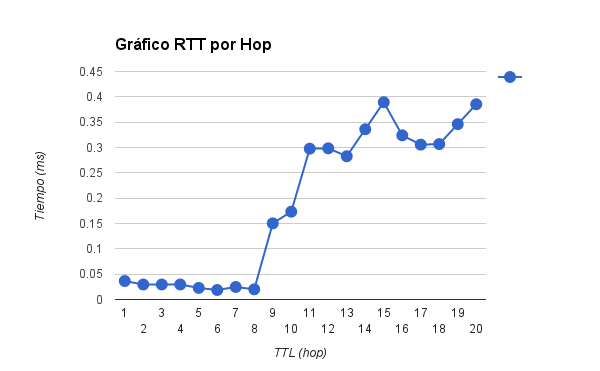
\includegraphics[width=0.7\textwidth]{img_analisis1/rtt_hop.png}
     %\label{fig:ICMPlista} 
	%\end{center} 
    
\end{figure}
\vspace{0.25cm}

%Promedio Delta RTT: 0.00588932037354, 0.223511198044, -0.0304053096771, -0.0112577915192, 0.0367794513702, 0.107529531662, -0.120579014962, 0.0107178688049, 0.107933545113, -0.0993495464325, 0.0167979955673, -0.0487000465393, 0.064146566391, 0.0933417320251, 0.0240439891815, -0.0125254392624, 0.0359566926956, -0.0348659515381, 0.0918450593948, -4.58002090454e-05, -0.00115667533875, 0.00671604824066, 0.0508928060532, -0.0580342292786, 0.00854189395905, 0.00741848945618, -0.143095983322, 0.102489104051\newline
\begin{figure}[h]
	%\begin{center}
    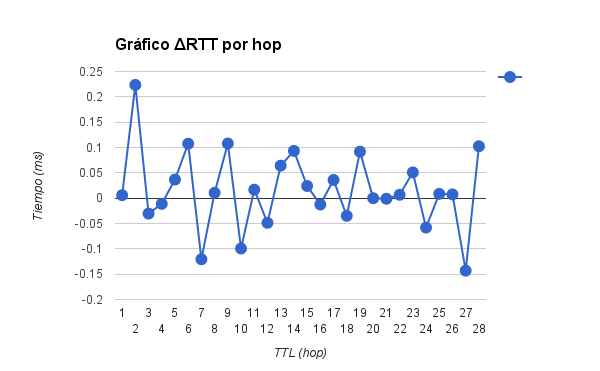
\includegraphics[width=0.7\textwidth]{img_analisis1/delta_rtt_hop.png}
     %\label{fig:ICMPlista} 
	%\end{center} 
    
\end{figure}
\vspace{0.25cm}

%Desvio Estandar Delta RTT: 0.00165442878817, 0.126023742282, 0.071172659274, 0.0745178056825, 0.1866931839, 0.180733182681, 0.0518781646894, 0.065719884364, 0.227576463877, 0.177889865429, 0.0311607993988, 0.0706603578755, 0.147728183499, 0.0762432009451, 0.0966932498659, 0.11828018604, 0.0873092181674, 0.0842616491826, 0.0484700197953, 0.112708845656, 0.0881211770851, 0.0889849976974, 0.0825379976568, 0.0601178559323, 0.0414772504639, 0.0872692906756, 0.0765956277221, 0.0546049405093\newline
\begin{figure}[h]
	%\begin{center}
    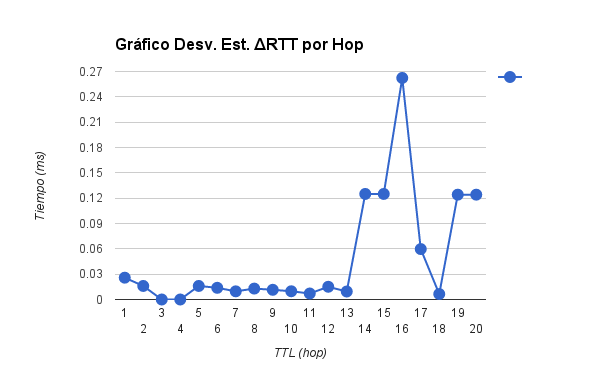
\includegraphics[width=0.7\textwidth]{img_analisis1/ds_delta_rtt_hop.png}
     %\label{fig:ICMPlista} 
	%\end{center} 
    
\end{figure}
\vspace{0.25cm}

De la muestra obtuvimos una distribuci\'on Normal, y los siguientes enlaces submarinos: nodo 2, nodo 5.\newline

Gr\'afico de mapa marcando puntos claves de la ruta:

\subsubsection{Conclusi\'on}
Explicaci\'on de los resultados obtenidos.
	\section{An\'alisis 2: Universidad de Sydney}
Vamos a realizar un an\'alisis de nuestro traceroute sobre la universidad de la capital australiana.\newline

El host de dicha universidad es http://sydney.edu.au/ (IP: 129.78.5.8).\\	

\subsubsection{Par\'ametros de entrada}
\begin{itemize}
\item Host: sydney.edu.au
\item Tiempo Limite: 5
\item Cant. Iteraciones en cada nodo: 10
\item Recorrido m\'aximo de nodos: 30 (TTL m\'aximo)
\item alpha: 0.05
\end{itemize}
El tiempo limite indica cuanto esperar de respuesta, como m\'aximo, a un nodo.\newline

\subsubsection{Resultados obtenidos}

Captura general de los resultados obtenidos: \newline


\begin{figure}[h]
	\begin{center}
    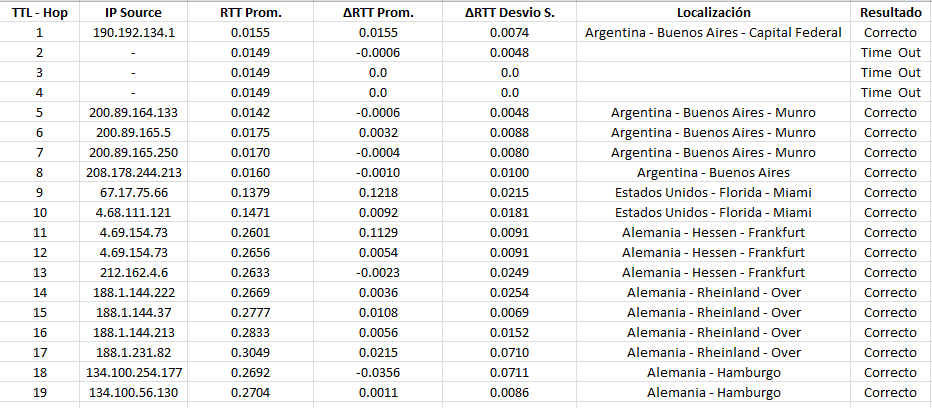
\includegraphics[width=1\textwidth]{img_analisis3/captura.png} 
	\end{center} 
\end{figure}
%TTL:  1    IP Source: 190.192.134.1    Argentina - Buenos Aires - Capital Federal\\ 
%TTL:  2    Obtuvimos time out, dado que el nodo 2 no contesto. \\
%TTL:  3    Obtuvimos time out, dado que el nodo 3 no contesto. \\
%TTL:  4    Obtuvimos time out, dado que el nodo 4 no contesto. \\
%TTL:  5    IP Source: 200.89.166.105   Argentina - Buenos Aires - Capital Federal\\  
%TTL:  6    IP Source: 200.89.165.197   Argentina - Buenos Aires - Capital Federal\\ 
%TTL:  7    IP Source: 200.89.165.222   Argentina - Buenos Aires - Capital Federal\\ 
%TTL:  8    IP Source: 208.178.244.213  EEUU - Kansas\\ 
%TTL:  9    IP Source: 67.16.139.18     EEUU - Illinois\\ 
%TTL: 10    IP Source: 129.250.9.117    EEUU - Colorado - Denver\\ 
%TTL: 11    IP Source: 129.250.3.172    EEUU - Colorado - Denver\\  
%TTL: 12    IP Source: 129.250.2.219    EEUU - Colorado - Denver\\ 
%TTL: 13    IP Source: 129.250.7.69     EEUU - Colorado - Denver\\ 
%TTL: 14    IP Source: 129.250.3.123    EEUU - Colorado - Denver\\  
%TTL: 15    IP Source: 204.1.253.166    EEUU - California - Los \'Angeles\\
%TTL: 16    IP Source: 202.158.194.172  Australia - Wahroonga\\ 
%TTL: 17    IP Source: 113.197.15.68    Australia - Wahroonga\\ 
%TTL: 18    IP Source: 113.197.15.66    Australia - Wahroonga\\  
%TTL: 19    IP Source: 113.197.15.62    Australia - Wahroonga\\  
%TTL: 20    IP Source: 113.197.15.13    Australia - Wahroonga\\  
%TTL: 21    IP Source: 138.44.5.47      Australia - Tamworth\\ 
%TTL: 22    Obtuvimos time out, dado que el nodo 22 no contesto. \\ 
%TTL: 23    Obtuvimos time out, dado que el nodo 23 no contesto. \\
%TTL: 24    IP Source: 129.78.5.8       Australia - Sydney\newline


De la muestra obtuvimos una distribuci\'on Normal, y los siguientes enlaces submarinos seg\'un el test de Grubbs: al pasar al nodo 9 y al pasar al nodo 16.\newline

\subsubsection{An\'alisis de los resultados}
Mediante gr\'aficos haremos un an\'alisis de los resultados obtenidos. \newline


\begin{figure}[h]
	\begin{center}
    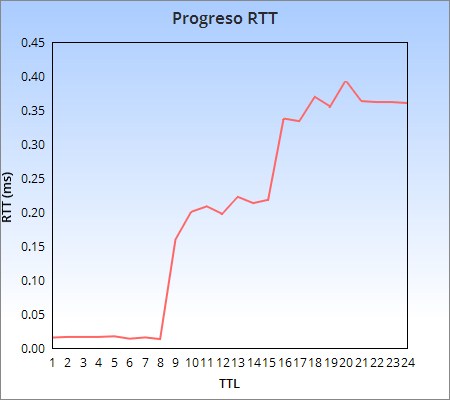
\includegraphics[width=0.7\textwidth]{img_analisis2/RTTprom.png} 
	\caption{Figura 1: Rtt promedio - Universidad de Sydney}	
	\end{center} 
	
    
\end{figure}



\begin{figure}[h]
	\begin{center}
    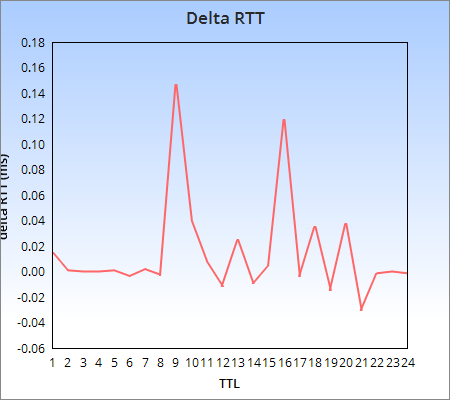
\includegraphics[width=0.7\textwidth]{img_analisis2/Delta_RTT.png}
     \caption{Figura 2: Delta RTT - Universidad de Sydney} 
	\end{center} 
    
\end{figure}
\vspace{0.25cm}


Podemos ver claramente en los gr\'aficos como en los saltos 9 y 16, que hab\'ian dado como outliers en el test de Grubbs, se denota un cambio brusco tanto en los RTT promedio como en los delta RTT. Con respecto al gr\'afico de RTT promedio podemos ver como de golpe en el salto 9, por ejemplo, sube de 0.013 a 0.15 mili segundos. Mientras tanto, en el gr\'afico de delta RTT, tambi\'en vemos un pico en los saltos marcados como outliers. En este caso se ven aun m\'as claro los outliers ya que se forman picos abruptos.\\
Como la ruta que hacen los paquetes es Argentina-EEUU-Australia, entonces deber\'iamos tener 2 grandes saltos en la traza: Desde Argentina a Estados Unidos (aunque no fuera un enlace submarino s\'i es considerable la distancia (9000 km)), y desde Estados Unidos hasta Australia (en este caso si es un enlace submarino). \newline

Viendo la locallizaci\'on de las ip y los saltos donde nos da el primer outlier, podemos notar que el hop que va desde la  ip 8 (208.178.244.213  EEUU - Kansas) hasta la ip 9 (67.16.139.18     EEUU - Illinois) en realidad no se mueve de Estados Unidos. Creemos que, en realidad, la ip correspondiente al salto n\'umero 8 se encuentra en Argentina pues los RTT de los saltos anteriores (5, 6 y 7), podemos suponer de que el router en realidad est\'a ubicado en alguna parte de Argentina o Sudam\'erica. Creemos que esto sucede porque es un router que brinda servicio a Estados Unidos pero en realidad est\'a f\'isicamente ubicado en Argentina o Sudam\'erica.  \newline

Con respecto al segundo outlier podemos decir que en esta ocaci\'on si se cumple nuestra hip\'otesis. Podemos ver que la ip 15 (204.1.253.166    EEUU - California - Los \'Angeles) se encuetra en el continente americano mientras que la ip 16 (202.158.194.172  Australia - Wahroonga) ya se encuentra en tierras oce\'anicas. \newline

Finalmente presentamos un mapa global donde vamos a trazar los puntos importantes de la ruta que realizan los paquetes. 




	\section{An\'alisis 3: Universidad de Hamburgo (Alemania)}
Vamos a realizar un an\'alisis de nuestro traceroute sobre la Universidad de Hamburgo.

El host de dicha universidad es http://www.uni-hamburg.de/ (IP: 134.100.56.130 ).\\	


\subsubsection{Par\'ametros de entrada}
\begin{itemize}
\item Host: www.uni-hamburg.de
\item Tiempo Limite: 2
\item Cant. Iteraciones en cada nodo: 15
\item Recorrido m\'aximo de nodos: 25 (TTL m\'aximo)
\item alpha: 0.05
\end{itemize}

\subsubsection{Resultados obtenidos}

Captura general de los resultados obtenidos: 
\\
\\

TTL:  1    IP Source: 190.192.134.1  Argentina - Buenos Aires - Capital Federal\\ 
TTL:  2    Obtuvimos time out, dado que el nodo 2 no contesto. \\
TTL:  3    Obtuvimos time out, dado que el nodo 3 no contesto. \\
TTL:  4    Obtuvimos time out, dado que el nodo 4 no contesto. \\
TTL:  5    IP Source: 200.89.164.133 Argentina - Buenos Aires - Munro\\  
TTL:  6    IP Source: 200.89.165.5 Argentina - Buenos Aires - Munro\\ 
TTL:  7    IP Source: 200.89.165.250 Argentina - Buenos Aires - Munro\\ 
TTL:  8    IP Source: 208.178.244.213 Argentina - Buenos Aires\\ 
TTL:  9    IP Source: 67.17.75.66 Estados Unidos - Florida - Miami\\ 
TTL: 10    IP Source: 4.68.111.121 Estados Unidos - Florida - Miami\\ 
TTL: 11    IP Source: 4.69.154.73 Alemania - Hessen - Frankfurt\\  
TTL: 12    IP Source: 4.69.154.73 Alemania - Hessen - Frankfurt\\ 
TTL: 13    IP Source: 212.162.4.6 Alemania - Hessen - Frankfurt\\ 
TTL: 14    IP Source: 188.1.144.222 Alemania - Rheinland-pfalz - Over\\  
TTL: 15    IP Source: 188.1.144.37 Alemania - Rheinland-pfalz - Over\\
TTL: 16    IP Source: 188.1.144.213 Alemania - Rheinland-pfalz - Over\\ 
TTL: 17    IP Source: 188.1.231.82 Alemania - Rheinland-pfalz - Over\\ 
TTL: 18    IP Source: 134.100.254.177 Alemania - Hamburgo - Hamburgo\\  
TTL: 19    IP Source: 134.100.56.130 Alemania - Hamburgo - Hamburgo\\ 
\newline

\subsubsection{An\'alisis de los resultados}
Mediante gr\'aficos haremos un an\'alisis de los resultados obtenidos. \newline

\begin{figure}[h]
	\begin{center}
    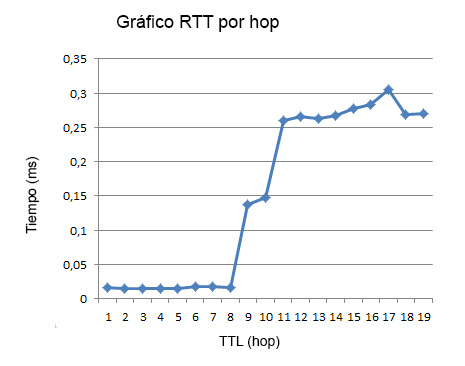
\includegraphics[width=0.7\textwidth]{img_analisis3/grafico-rtt-promedio.jpg} 
    \caption{Figura 1: $RTT$ promedio - Universidad de Hamburgo}	
	\end{center} 
\end{figure}

\begin{figure}[h]
	\begin{center}
    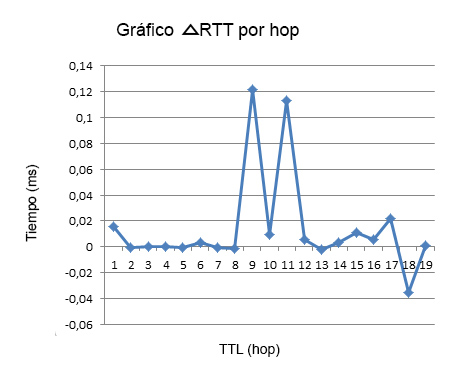
\includegraphics[width=0.7\textwidth]{img_analisis3/grafico-delta-rtt-promedio.jpg} 
    \caption{Figura 1: $\Delta RTT$ promedio - Universidad de Hamburgo}	
	\end{center} 
\end{figure}
%\newline
\newpage

De la muestra obtuvimos que los $\Delta RTT$ sigen una distribuci\'on Normal y que los enlaces submarinos, según los outliers obtenidos mediante el test de Grubbs, se corresponden con el salto 9 y el 11.
\\
Al observar los gráficos podemos notar que los resultados obtenidos mediante el test de Grubbs son correctos, ya que del salto 8 al 9 el paquete enviado viaja, según la geolocalización de las IP, desde Buenos Aires a Miami y su RTT promedio aumenta significativamente, y del salto 10 al 11 el paquete viaja de Miami a Frankfurt donde también hay un cambio abruto de su RTT promedio.
\\
Finalmente presentamos un mapa global donde vamos a trazar los puntos importantes de la ruta que realizan los paquetes. 
\newpage
\begin{figure}[h]
	\begin{center}
    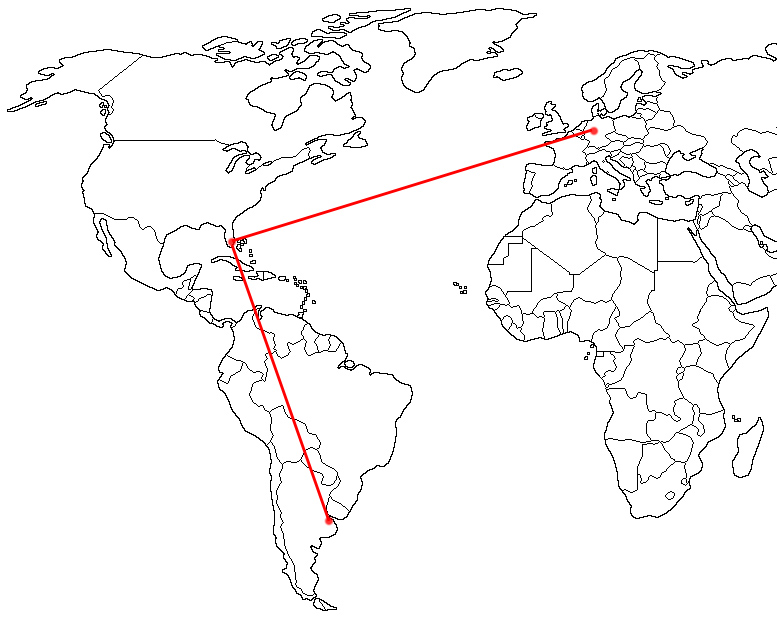
\includegraphics[width=0.7\textwidth]{img_analisis3/mapa.jpg} 
    \caption{Figura 1: Ruta del paquete - Universidad de Hamburgo}	
	\end{center} 
\end{figure}


	\newpage

\end{document}

